\documentclass[../em.tex]{subfiles}
\graphicspath{{\subfix{../figures/}}}
\begin{document}
\chapter{Electric Potential}
\section{Electric Potential Energy}
The electric potential energy of a system of two point charges equals the amount of 
work required for an external force to bring point charges to their 
current positions from infinitely far away.

The general form of the electric potential energy between
two charged objects is given by the equation:
\[U=\frac{kq_1q_2}{r}=\frac{1}{4\pi\epsilon_0}\cdot\frac{q_1q_2}{r}\]

The total electric potential energy of a system can be determined by 
finding the sum of the electric potential energies of the individual
interactions between each pair of charged objects in the system.

When there are opposite signs, the $U$ value will decrease when close together.

When there are same signs, the $U$ value will increase when close together.

\begin{example}
    Derive an expression for the work required to assemble the charges
    in the configuration shown.
    \begin{center}
        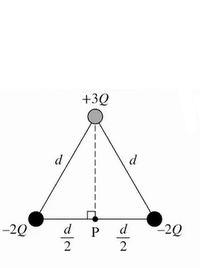
\includegraphics[width=0.3\textwidth]{9.1.PNG}
    \end{center}

    Remember that
    \[W = \Delta U = \sum U\]
    
    So we have:
    \[\frac{kq_1q_2}{d}+\frac{kq_1q_3}{d}+\frac{kq_2q_3}{d}=\\
    k\left[\frac{(-2Q)(3Q)}{d}+\frac{(-2Q)(-2Q)}{d}+\frac{(-2Q)(3Q)}{d}\right]\\
    =8Q\]
\end{example}

\ex Two point charges, one with positive charge $+2Q$ and one with negative charge $-Q$, are fixed in a distance $D$ apart. The electric potential energy of the two-point charge system is $U_0$. If a third, positive, point charge is added to the system,
where should the point charge be located so that the electric potential energy of the three-point charge system is still $U_0$? What evidence or reasoning supports the claim?

\ex Consider four different systems consisting of a pair of point charges. The point charges in the systems have the following charge values and separation distances.
\begin{itemize}
    \item System 1: point charges of +1 nC and +1 nC, separated by 1 cm 
    \item System 2: point charges of +1 nC and +4 nC, separated by 4 cm 
    \item System 3: point charges of -1 nC and +6 nC, separated by 1 cm 
    \item System 4: point charges of +2 nC and +2 nC, separated by 2 cm
\end{itemize}
Which of the following correctly ranks the electric potential energies $U_1$, $U_2$, $U_3$. and $U_4$ of the four systems. Take the potential energy of a system to be zero when the point charges are infinitely apart.

\ex A system is comprised of two positive point charges, which have charge values of 1 nC and 2 nC. How does the amount of work done on the system by an external force or forces for the following three scenarios?
\begin{itemize}
    \item Scenario 1: $W_1$ is the work done by an external force to move the 1 nC point charge from far away to a distance of 1 cm from the 2 nC point charge, which is fixed in place.
    \item Scenario 2: $W_2$ is the work done by an external force to move the 2 nC point charge from far away to a distance of 1 cm from the 1 nC point charge, which is fixed in place.
    \item Scenario 3: $W_3$ is the total work done by external forces to move both point charges simultaneously from far away to locations that are a distance of 1 cm from each other.
\end{itemize}
In each scenario, the initial positions of any point charges that get moved can be considered to be infinitely far away.

\section{Electric Potential}
Electric potential describes the electric potential energy per unit of charge at a point in space.

Expressions for the electric potential of charge distributions can be found by
using integration and the principle of superposition:
\[V=\frac{1}{4\pi\epsilon_0}\int \frac{\mathrm{d}q}{r}\]

If there are multiple point charges, we just add up all the point charges.

The electric potential difference between two points is the change in the electric potential energy
per unit charge when a test charge is moved between two points:
\[\Delta{V}=\frac{\Delta{U_E}}{q}\]

The value of the electric field component in any direction at a given point is equal to the 
negative of the rate of change in electric potential at that location:
\[E_x=-\mathrm{d}V/\mathrm{d}x\]

The change in electric potential between two points can be determined by integrating the dot product
of the electric field and the displacement along the path connecting the points:
\[\Delta{V}=V_b-V_a=-\int{\vec{E}\cdot\mathrm{d}\vec{r}}\]

Equipotential lines represent lines of equal potential energy. These lines are perpendicular to the electric field vectors.
Electric field vectors point in the direction of decreasing potential. There is no component of an electric field along an equipotential line.

\begin{example}
    Derive an expression for the absolute value of the potential difference between the outer surface
    of the sphere and the inner surface of the shell. Express your answer in terms of $Q$, $R$, and physical constants,
    as appropriate.

    \begin{center}
        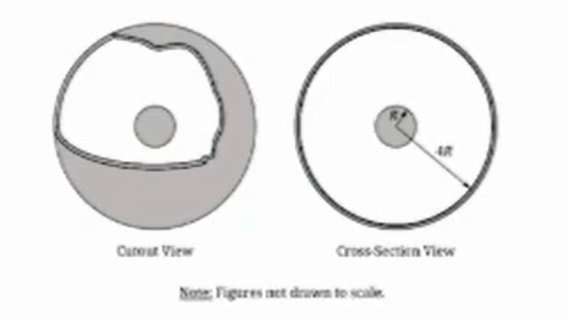
\includegraphics[width=0.3\textwidth]{9.2.PNG}
    \end{center}

    Previously we would have found the electric field is:
    \[E=-\frac{Q}{4\pi\epsilon_0r^2}\]

    So we must integrate:
    \begin{align*}
    \Delta V=-\int_R^{4R}\vec{E}\cdot\mathrm{d}\vec{R} \\
    \Delta V = +\int_R^{4R}+\frac{Q}{4\pi\epsilon_0 r^2}\mathrm{d}r\\
    \Delta V = \frac{Q}{4\pi\epsilon_0}\int_R^{4R}\frac{\mathrm{d}r}{r^2}\\
    \Delta V = \frac{Q}{4\pi\epsilon_0}\left[+\frac{1}{r}\right]
    \end{align*}
    Applying the limits of integration we get: 
    \[\Delta V = \frac{3Q}{4\pi\epsilon_0 R}\]
\end{example}

\ex Two point charges are located on the $x$-axis. A -4.0 nC point charge is at $x=-0.20$ m, and a $+5.0$ nC point charge is at $x=+0.10$ m. What is the electric potential on the $x$-axis at $x=0.00$ m? Take the potential to be zero at an infinite distance from the point charges.

\section{Conservation of Electric Energy}
When a charged object moves between two locations with different electric potentials, the resulting change in the electric potential energy
of the object-field system is given by:
\[\Delta U_E=q\Delta V\]

The movement of a charged object between two points with different electric potential results in a change in kinetic
energy of the object consistent with the conservation of energy.

\begin{example}
    A proton (mass $=1.67\times10^{-27}$ kg) is accelerated through a potential difference of $4.5\times10^6$ V.
    (a) How much kinetic energy has the proton acquired? (b) If the proton started at rest, how fast is it moving.

    For part A, we have
    \begin{align*}
    \Delta U = q\Delta V = \Delta K = K-K_0 \\
    = (1.6\times10^{-19})(4.5\times10^6\text{V})\\
    = 7.2\times10^{-13}\text{J}
    \end{align*}

    For part B:
    \begin{align*}
        K = \frac{1}{2}mv^2\\
        V = \sqrt{\frac{2K}{m}}\\
        = \sqrt{\frac{2(7.2\times10^{-13})}{1.67\times10^{-27}}}=2.94\times10^7\text{m/s}
    \end{align*}
    
\end{example}
\ex A proton in an electric field is initially located at point $P_1$ on the $x$-axis. The proton is given an initial velocity in the positive $x$-direction, moves in a straight line along the axis, and 
continually slows down and comes instantaneously to rest at point $P_2$. What can be concluded about the electric potential at points $P_1$ and $P_2$, and what evidence or reasoning supports the claim?

\ex An electron is accelerated from rest through a potential difference of $\delta V_0$, reaching a speed of $v_1$. A different electron is accelerated from rest through a potential difference of $4\delta V_0$, reaching a speed of $v_2$. The ratio of $\frac{v_2}{v_1}$ is?



\end{document}